\documentclass{article}
\usepackage[margin=1in]{geometry}
\usepackage{amsmath,amsthm,amssymb}
\usepackage{bbm,enumerate,mathtools}
\usepackage{tikz,pgfplots}
\usepackage{chessboard}
\usepackage[hidelinks]{hyperref}
\usepackage{multicol} % Problem 35

\newenvironment{question}{\begin{trivlist}\item[\textbf{Question.}]}{\end{trivlist}}
\newenvironment{note}{\begin{trivlist}\item[\textbf{Note.}]}{\end{trivlist}}
\newenvironment{references}{\begin{trivlist}\item[\textbf{References.}]}{\end{trivlist}}
\newenvironment{related}{\begin{trivlist}\item[\textbf{Related.}]\end{trivlist}\begin{enumerate}}{\end{enumerate}}


\begin{document}
  Consider square, triangular, and hexagonal grids that are filled in with
  with tiles of different patterns.
\begin{figure}[!h]
  \centering
  \begin{multicols}{2}\begin{itemize}
    % 1
    \item \leavevmode\vadjust{\vspace{-\baselineskip}}\newline
    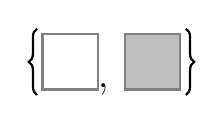
\begin{tikzpicture}[scale=0.7]
      \fill[gray!50] (1.5,0) rectangle (2.5,1);

      \def\count{1}
      \foreach \x in {0,...,\count} {\draw[gray, thick] (1.5*\x, 0) rectangle (1.5*\x + 1, 1);}
      \foreach \x in {1,...,\count} {\node at (1.5*\x - 0.4,0) {\Large,};}
      \draw [thick,decorate,decoration={brace,amplitude=3pt}] (-0.1,-0.1)--(-0.1,1.1);
      \draw [thick,decorate,decoration={brace,amplitude=3pt,mirror}] ({1.5*\count + 1.1},-0.1)--({1.5*\count + 1.1},1.1);
    \end{tikzpicture}
    % 2
    \item \leavevmode\vadjust{\vspace{-\baselineskip}}\newline
    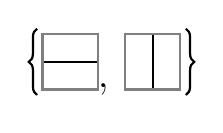
\begin{tikzpicture}[scale=0.7]
      \draw[thick] (0,0.5)--(1,0.5);
      \draw[thick] (2,0)--(2,1);

      \def\count{1}
      \foreach \x in {0,...,\count} {\draw[gray, thick] (1.5*\x, 0) rectangle (1.5*\x + 1, 1);}
      \foreach \x in {1,...,\count} {\node at (1.5*\x - 0.4,0) {\Large,};}
      \draw [thick,decorate,decoration={brace,amplitude=3pt}] (-0.1,-0.1)--(-0.1,1.1);
      \draw [thick,decorate,decoration={brace,amplitude=3pt,mirror}] ({1.5*\count + 1.1},-0.1)--({1.5*\count + 1.1},1.1);
    \end{tikzpicture}
    % 3
    \item \leavevmode\vadjust{\vspace{-\baselineskip}}\newline
    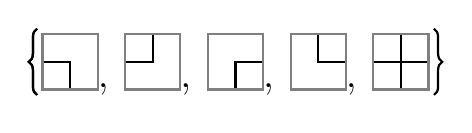
\begin{tikzpicture}[scale=0.7]
      \draw [thick,decorate,decoration={brace,amplitude=3pt}] (-0.1,-0.1)--(-0.1,1.1);
      \draw[thick] (0,0.5)--(0.5,0.5)--(0.5,0);
      \draw[thick] (1.5,0.5)--(2,0.5)--(2,1);
      \draw[thick] (3.5,0)--(3.5,0.5)--(4,0.5);
      \draw[thick] (5,1)--(5,0.5)--(5.5,0.5);
      \draw[thick] (6,0.5)--(7,0.5); \draw[thick] (6.5,0)--(6.5,1);

      \def\count{4}
      \foreach \x in {0,...,\count} {\draw[gray, thick] (1.5*\x, 0) rectangle (1.5*\x + 1, 1);}
      \foreach \x in {1,...,\count} {\node at (1.5*\x - 0.4,0) {\Large,};}
      \draw [thick,decorate,decoration={brace,amplitude=3pt}] (-0.1,-0.1)--(-0.1,1.1);
      \draw [thick,decorate,decoration={brace,amplitude=3pt,mirror}] ({1.5*\count + 1.1},-0.1)--({1.5*\count + 1.1},1.1);
    \end{tikzpicture}
    % 4
    \item \leavevmode\vadjust{\vspace{-\baselineskip}}\newline
    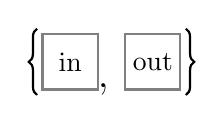
\begin{tikzpicture}[scale=0.7]
      \node at (0.5, 0.5) {in}; \node at (2, 0.5) {out};

      \def\count{1}
      \foreach \x in {0,...,\count} {\draw[gray, thick] (1.5*\x, 0) rectangle (1.5*\x + 1, 1);}
      \foreach \x in {1,...,\count} {\node at (1.5*\x - 0.4,0) {\Large,};}
      \draw [thick,decorate,decoration={brace,amplitude=3pt}] (-0.1,-0.1)--(-0.1,1.1);
      \draw [thick,decorate,decoration={brace,amplitude=3pt,mirror}] ({1.5*\count + 1.1},-0.1)--({1.5*\count + 1.1},1.1);
    \end{tikzpicture}
    % 5
    \item \leavevmode\vadjust{\vspace{-\baselineskip}}\newline
    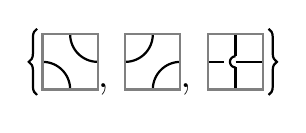
\begin{tikzpicture}[scale=0.7]
      \foreach \a/\b/\theta in {0/0/0, 1/1/180, 1.5/1/270, 2.5/0/90} {
        \draw[thick, draw={}, domain=\theta:\theta+90] plot ({0.5*cos(\x) + \a}, {0.5*sin(\x) + \b});
      }
      \draw[thick, domain=90:270] plot ({0.1*cos(\x) + 3.5}, {0.1*sin(\x) + 0.5});
      \draw[thick] (3.5,1)--(3.5,0.6); \draw[thick] (3.5,0.4)--(3.5,0);
      \draw[thick] (3,0.5)--(3.3,0.5); \draw[thick] (3.5,0.5)--(4,0.5);

      \def\count{2}
      \foreach \x in {0,...,\count} {\draw[gray, thick] (1.5*\x, 0) rectangle (1.5*\x + 1, 1);}
      \foreach \x in {1,...,\count} {\node at (1.5*\x - 0.4,0) {\Large,};}
      \draw [thick,decorate,decoration={brace,amplitude=3pt}] (-0.1,-0.1)--(-0.1,1.1);
      \draw [thick,decorate,decoration={brace,amplitude=3pt,mirror}] ({1.5*\count + 1.1},-0.1)--({1.5*\count + 1.1},1.1);
    \end{tikzpicture}
    % 6
    \item \leavevmode\vadjust{\vspace{-\baselineskip}}\newline
    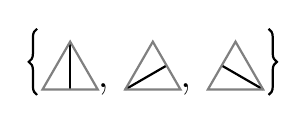
\begin{tikzpicture}[scale=0.7]
      \draw[thick] (0.5,0)--(0.5,{sqrt(3)/2});
      \draw[thick] (1.5,0)--(2.25,{sqrt(3)/4});
      \draw[thick] (4,0)--(3.25,{sqrt(3)/4});

      \def\count{2}
      \foreach \x in {0,...,\count} {\draw[gray, thick] (1.5*\x, 0)--(1.5*\x + 0.5, {sqrt(3)/2})--(1.5*\x + 1,0)--cycle;}
      \foreach \x in {1,...,\count} { \node at (1.5*\x - 0.4,0) {\Large,};}
      \draw [thick,decorate,decoration={brace,amplitude=3pt,mirror}] ({1.5*\count + 1.1},-0.1)--({1.5*\count + 1.1},1.1);
      \draw [thick,decorate,decoration={brace,amplitude=3pt}] (-0.1,-0.1)--(-0.1,1.1);
    \end{tikzpicture}
    % 7
    \item \leavevmode\vadjust{\vspace{-\baselineskip}}\newline
    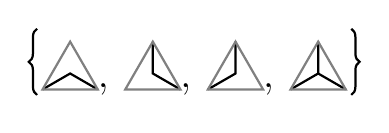
\begin{tikzpicture}[scale=0.7]
      \draw[thick] (0,0)--(0.5,{sqrt(3)/6})--(1,0);
      \draw[thick] (2,{sqrt(3)/2})--(2,{sqrt(3)/6})--(2.5,0);
      \draw[thick] (3,0)--(3.5,{sqrt(3)/6})--(3.5,{sqrt(3)/2});
      \draw[thick] (4.5,0)--(5,{sqrt(3)/6})--(5,{sqrt(3)/2}); \draw[thick] (5,{sqrt(3)/6})--(5.5,0);

      \def\count{3}
      \foreach \x in {0,...,\count} {\draw[gray, thick] (1.5*\x, 0)--(1.5*\x + 0.5, {sqrt(3)/2})--(1.5*\x + 1,0)--cycle;}
      \foreach \x in {1,...,\count} { \node at (1.5*\x - 0.4,0) {\Large,};}
      \draw [thick,decorate,decoration={brace,amplitude=3pt,mirror}] ({1.5*\count + 1.1},-0.1)--({1.5*\count + 1.1},1.1);
      \draw [thick,decorate,decoration={brace,amplitude=3pt}] (-0.1,-0.1)--(-0.1,1.1);
    \end{tikzpicture}
    % 8
    \item \leavevmode\vadjust{\vspace{-\baselineskip}}\newline
    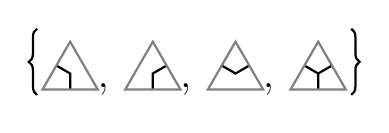
\begin{tikzpicture}[scale=0.7]
      \draw[thick] (0.25,{sqrt(3)/4})--(0.5,{sqrt(3)/6})--(0.5,0);
      \draw[thick] (2.25,{sqrt(3)/4})--(2,{sqrt(3)/6})--(2,0);
      \draw[thick] (3.75,{sqrt(3)/4})--(3.5,{sqrt(3)/6})--(3.25,{sqrt(3)/4});
      \draw[thick] (5.25,{sqrt(3)/4})--(5,{sqrt(3)/6})--(5,0); \draw[thick] (4.75,{sqrt(3)/4})--(5,{sqrt(3)/6});

      \def\count{3}
      \foreach \x in {0,...,\count} {\draw[gray, thick] (1.5*\x, 0)--(1.5*\x + 0.5, {sqrt(3)/2})--(1.5*\x + 1,0)--cycle;}
      \foreach \x in {1,...,\count} { \node at (1.5*\x - 0.4,0) {\Large,};}
      \draw [thick,decorate,decoration={brace,amplitude=3pt,mirror}] ({1.5*\count + 1.1},-0.1)--({1.5*\count + 1.1},1.1);
      \draw [thick,decorate,decoration={brace,amplitude=3pt}] (-0.1,-0.1)--(-0.1,1.1);
    \end{tikzpicture}
    % 9
    \item \leavevmode\vadjust{\vspace{-\baselineskip}}\newline
    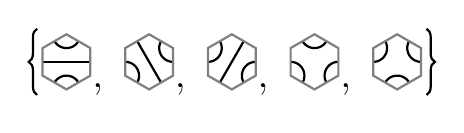
\begin{tikzpicture}[scale=0.7]
      \draw[thick, draw={}, domain=210:330] plot ({0.25*cos(\x) + sqrt(3)/4}, {0.25*sin(\x) + 1});
      \draw[thick, draw={}, domain=30:150] plot ({0.25*cos(\x) + sqrt(3)/4}, {0.25*sin(\x) + 0});
      \draw[thick] (0,0.5)--({sqrt(3)/2},0.5);

      \draw[thick, draw={}, domain=-30:90] plot ({0.25*cos(\x) + 1.5}, {0.25*sin(\x) + 0.25});
      \draw[thick, draw={}, domain=150:270] plot ({0.25*cos(\x) + 1.5 + sqrt(3)/2}, {0.25*sin(\x) + 0.75});
      \draw[thick] ({1.5 + sqrt(3)/8},{7/8})--({1.5 + 3*sqrt(3)/8},{1/8});

      \draw[thick, draw={}, domain=-90:30] plot ({0.25*cos(\x) + 3}, {0.25*sin(\x) + 0.75});
      \draw[thick, draw={}, domain=90:210] plot ({0.25*cos(\x) + 3 + sqrt(3)/2}, {0.25*sin(\x) + 0.25});
      \draw[thick] ({3 + 3*sqrt(3)/8},{7/8})--({3 + sqrt(3)/8},{1/8});

      \draw[thick, draw={}, domain=210:330] plot ({0.25*cos(\x) + 4.5 + sqrt(3)/4}, {0.25*sin(\x) + 1});
      \draw[thick, draw={}, domain=-30:90] plot ({0.25*cos(\x) + 4.5}, {0.25*sin(\x) + 0.25});
      \draw[thick, draw={}, domain=90:210] plot ({0.25*cos(\x) + 4.5 + sqrt(3)/2}, {0.25*sin(\x) + 0.25});

      \draw[thick, draw={}, domain=30:150] plot ({0.25*cos(\x) + 6 + sqrt(3)/4}, {0.25*sin(\x) + 0});
      \draw[thick, draw={}, domain=-90:30] plot ({0.25*cos(\x) + 6}, {0.25*sin(\x) + 0.75});
      \draw[thick, draw={}, domain=150:270] plot ({0.25*cos(\x) + 6 + sqrt(3)/2}, {0.25*sin(\x) + 0.75});

      \def\count{4}
      \foreach \x in {0,...,\count} {\draw[gray, thick] (1.5*\x, 1/4)--(1.5*\x, 3/4)--({1.5*\x + sqrt(3)/4}, 1)--({1.5*\x + sqrt(3)/2}, 3/4)--({1.5*\x + sqrt(3)/2}, 1/4)--({1.5*\x + sqrt(3)/4}, 0)--cycle;}
      \foreach \x in {1,...,\count} {\node at (1.5*\x - 0.5,0) {\Large,};}
      \draw [thick,decorate,decoration={brace,amplitude=3pt}] (-0.1,-0.1)--(-0.1,1.1);
      \draw [thick,decorate,decoration={brace,amplitude=3pt,mirror}] ({1.5*\count + 0.1 + sqrt(3)/2},-0.1)--({1.5*\count + 0.1 + sqrt(3)/2},1.1);
    \end{tikzpicture}
    % 10
    \item \leavevmode\vadjust{\vspace{-\baselineskip}}\newline
    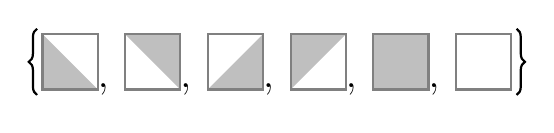
\begin{tikzpicture}[scale=0.7]
      \fill[gray!50] (0,0)--(0,1)--(1,0)--cycle;
      \fill[gray!50] (2.5,1)--(1.5,1)--(2.5,0)--cycle;
      \fill[gray!50] (3,0)--(4,1)--(4,0)--cycle;
      \fill[gray!50] (3,0)--(4,1)--(4,0)--cycle;
      \fill[gray!50] (4.5,0)--(4.5,1)--(5.5,1)--cycle;
      \fill[gray!50] (6,0) rectangle (7,1);

      \def\count{5}
      \foreach \x in {0,...,\count} {\draw[gray, thick] (1.5*\x, 0) rectangle (1.5*\x + 1, 1);}
      \foreach \x in {1,...,\count} {\node at (1.5*\x - 0.4,0) {\Large,};}
      \draw [thick,decorate,decoration={brace,amplitude=3pt}] (-0.1,-0.1)--(-0.1,1.1);
      \draw [thick,decorate,decoration={brace,amplitude=3pt,mirror}] ({1.5*\count + 1.1},-0.1)--({1.5*\count + 1.1},1.1);
    \end{tikzpicture}
  \end{itemize}\end{multicols}
  \caption{Ten examples of different tiles.}
\end{figure}

\begin{question}
  How many essentially different grids of size $n$ exist with these tiles?
  (Up to dihedral action? Up to cyclic action?)
\end{question}
\begin{related}
  \item The square grid can be $n \times n$ or $n \times m$.
  \item The hexagonal grid can have triangles with side length $n$ or hexagons with side length $n$.
  \item The triangular grid can have triangles with side length $n$ or hexagons with side length $n$.
  \item The square grid can be quotiented to be a cylinder, torus, or M\"obius strip.
  \item What if shapes have to ``match-up'' (e.g. the lines in the third example
    or colors in the last example have to be ``smooth''.)
  \item How many distinct regions, as in Question 3?
\end{related}
\begin{references}
  \item Question 3.
  \item Question 32.
  \item \url{https://en.wikipedia.org/wiki/Burnside%27s_lemma}
\end{references}

\end{document}
